\documentclass[12pt]{article}
\usepackage{amsmath}
\usepackage{amssymb}
\usepackage{amsthm}
\usepackage{float}
\usepackage{subcaption}
\usepackage{caption}
\usepackage{enumerate,proof,color}
\usepackage{graphicx}

\title{Software Architecture Document\\Version 2.0}

\begin{document}
\maketitle

\section*{Reversion History}
\section*{Key Word} Image Inpainting Software, Architecture, Design, Software Structure
\section*{Abstract}
\qquad This document is used to describe the software architecture of our image inpainting software. It is the guideline of our software developing and structure. We will illustrate clearly how we design and implement our image inpainting software. In this document , we will describe the detailed design idea and reader can have a clear picture with referring to the rational rose design model.

\newpage
\tableofcontents
\newpage

\section{Introduction}
\subsection{Purpose}
\qquad This document is the guideline of our software developing and structure. Tt provides a comprehensive architectural overview of our image inpainting software.  It uses a number of different architectural views to depict different aspects of the system to help illustrate the software architecture. In this document , we will describe the detailed design idea and reader can have a clear picture with referring to the rational rose design model. It is intended to capture and convey the significant architectural decisions.
\subsection{Scope}
\qquad This document is an overview of the architecture and how it should be modeled. Decisions in this document affect how the system is modeled. Implementations of software is supposed to accord to this document.

\section{Architectural Representation}
\qquad In this document, the architecture of the application is represented following the recommendations of the Rational Unified Process and the Rational Architecture Practice guidelines. 

Our image inpainting software implemented two different algorithm and users can choose different method to satisfy their requirement. In other document, we will illustrate clearly the detail algorithm of these two method. And in this document, we will describe the software architecture of our image inpainting software.

This document presents the architectural as a series of views:

\begin{enumerate}
	\item Use-Case View
	\item Logical View
	\item Process Vied
	\item Implement View
	\item Deploy View
\end{enumerate}


\section{Use-Case View}
\subsection{Overview}
\qquad The Use Case View is important input to the selection of the set of scenarios and/or use cases that are the focus of an iteration. 

Our image inpainting software provide users freedom to choose the input image and the input mask. Users can choose their wanted area in the input image and our image inpainting software will inpaint the target area.There are different applicable scenario for out software including image text removal, object removal and image detail restoration etc. We also provide the users the UI to satisfy their requirements. 

All implemented use cases also have an associated Us-Case Specification document. You can refer to the Use-Case Specification document and get more details.

The functionality of our image inpainting software is captured in the Use-Case graph below:
\begin{figure}[H]
	\centering
	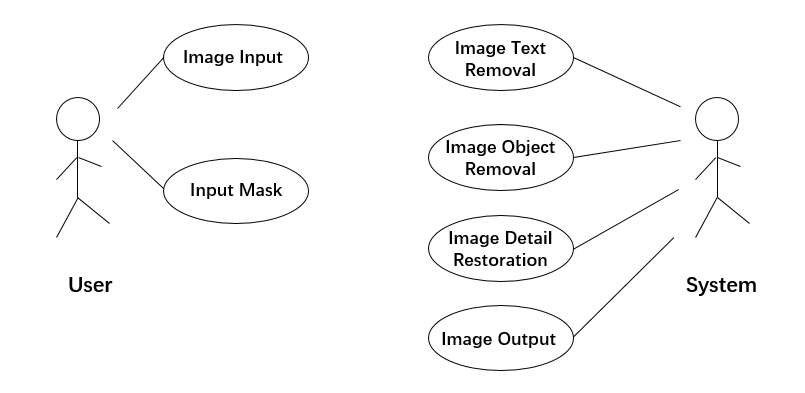
\includegraphics[width=1.0\linewidth]{use-case.jpg}
	\caption{Use-Case View}
\end{figure}

\subsection{Applicable Scenario}
\subsection{Architecturally-Significant Use Cases}

\section{Logical View}
\qquad In this section, we will describes the architecturally significant parts of the design model, such as its decomposition into subsystems and packages. This section will illustrate clearly the logical structure of the system. It presents its key structure, behavioral elements and and related structure.

There are three dominant structures in the application design model:
\begin{enumerate}
	\item Logical decomposition of the system into three layers.
	\item The structure of the use case realizations derived from model templates of architectural mechanisms.
	\item The design mechanisms package contains the a pre-designed solution to a common problem. 
\end{enumerate}

The high-level diagram of above is showed in the following graph:
\begin{figure}[H]
	\centering
	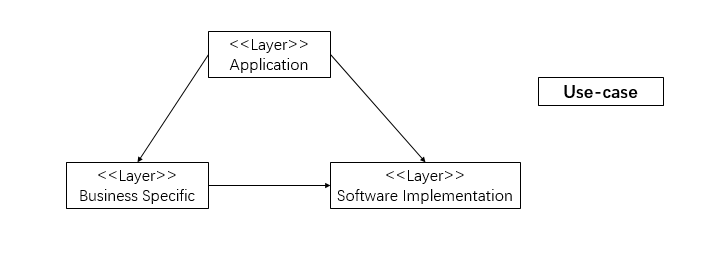
\includegraphics[width=1.0\linewidth]{logical.jpg}
	\caption{Logical View}
\end{figure}


In the logical view graph, It include three soft ware layers and the Use-Case realizations. These are illustrate below:
\begin{enumerate}
	\item Application: This layer is for special logic. It has a close relation to the presentation logic. The boundary classes are contained in this layer. It includes our two different implementation algorithm: Markov random field and exemplar-based algorithm.
	\item Business Specific: This layer includes business components and one common elements and services component. The components in this layer have a high reusability. It can be reuse in other situation or development process.
	\item Software Implementation: This layer includes some basic implementation of our image inpainting software. It include the platform and the detail language of our software. In our image inpainting software, we use MatLab and Python as our development language, and use Ubuntu 16.04 and Windows 10 as our development platform.
	\item Use-Case: It include the detail use-case situation of our image inpainting software.
\end{enumerate}

\section{Process View}
\qquad In our image inpainting software, there are total one process. Users choose the image that they want to inpaint and the mast which covers the target area, then they can click the button in our UI. Then they will get the result. 

The detail process will describe in the following graph:
\begin{figure}[H]
	\centering
	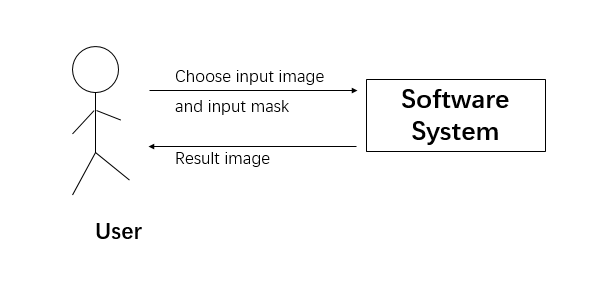
\includegraphics[width=1.0\linewidth]{process.jpg}
	\caption{Process View}
\end{figure}

In the process, it includes the following steps:
\begin{enumerate}
	\item Users choose the image that they want to inpaint and the mast
	\item Our image inpainting software system will process the input image and input mask.
	\item Software system presents the result image to users. 
\end{enumerate}

\section{Development View}
\qquad The deployment view of a system shows the physical nodes on which the system executes and the assignment of the system processed to the nodes. 

The diagram below shows the most typical deployment configuration used by the development team.
\begin{figure}[H]
	\centering
	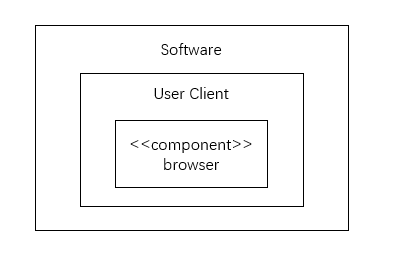
\includegraphics[width=0.8\linewidth]{develop.jpg}
	\caption{Development View}
\end{figure}


\section{Implement View}
\qquad This section include our development platform and our development language. Due to we implement two different algorithm, so we use different platform and development tools.

The detail is shown in the following graph:
\begin{figure}[H]
	\centering
	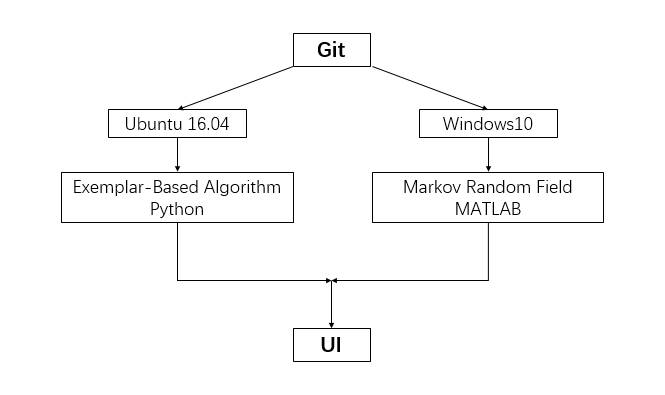
\includegraphics[width=1.0\linewidth]{implement.jpg}
	\caption{Implement View}
\end{figure}
As is shown in the graph, we use different tools to help our development including:
\begin{enumerate}
	\item Git: It is a version control system for tracking changes in computer files and coordinating work on those files among multiple people. It is primarily used for software development, but it can be used to keep track of changes in any files. As a distributed revision control system it is aimed at speed, data integrity, and support for distributed, non-linear workflows. We use Git to manage our software version and and tracking changes, which can support our development in different platform.
	\item MatLab: MATLAB (matrix laboratory) is a multi-paradigm numerical computing environment and fourth-generation programming language. A proprietary programming language developed by MathWorks, MATLAB allows matrix manipulations, plotting of functions and data, implementation of algorithms, creation of user interfaces, and interfacing with programs written in other languages. We use MatLab to implement our Markov Random Field Algorithm, which is much more convenient doing matrix operation.
	\item Python: Python is a widely used high-level programming language used for general-purpose programming. It can provide us some basic image process library.We use python to implement our Exemplar-Based Algorithm and our final UI.
\end{enumerate}
\section{Reference}


\newpage
% sample citation
Cite a paper\cite{DBLP:conf/siggraph/BertalmioSCB00}
\bibliography{report}
\bibliographystyle{abbrv}


\end{document}
